\chapter{Application Development}\label{ch:applications}

This chapter details the development of our two application frontends: the React Native mobile voting app (for citizens) and the Next.js web application (for administrators, GN officers, and public observers). We describe the architecture of each, focusing on the security-critical flows: hardware keystore management, biometric authentication, on-device proof generation, and the three-factor voting protocol.

\section{Mobile Application Architecture}

\subsection{Technology Stack}

\begin{table}[H]
\centering
\caption{Mobile application technology stack.}
\label{tab:mobile-stack}
\begin{tabular}{|l|l|l|}
\hline
\textbf{Component} & \textbf{Technology} & \textbf{Version} \\
\hline
Framework & React Native & 0.81.5 \\
\hline
Platform & Expo & SDK 54 \\
\hline
JS Engine & Hermes & (bundled) \\
\hline
Routing & Expo Router & v6 \\
\hline
EVM Interaction & viem & 2.21.0 \\
\hline
Cryptography & poseidon-lite & 0.3.0 \\
\hline
Key Storage & expo-secure-store & 15.0.8 \\
\hline
Biometrics & expo-local-authentication & 17.0.8 \\
\hline
QR Display & react-native-qrcode-svg & 6.3.2 \\
\hline
Merkle Tree & @zk-kit/lean-imt & 2.2.4 \\
\hline
\end{tabular}
\end{table}

\subsection{Screen Architecture}

The mobile app uses Expo Router's file-based routing:

\begin{figure}[H]
\centering
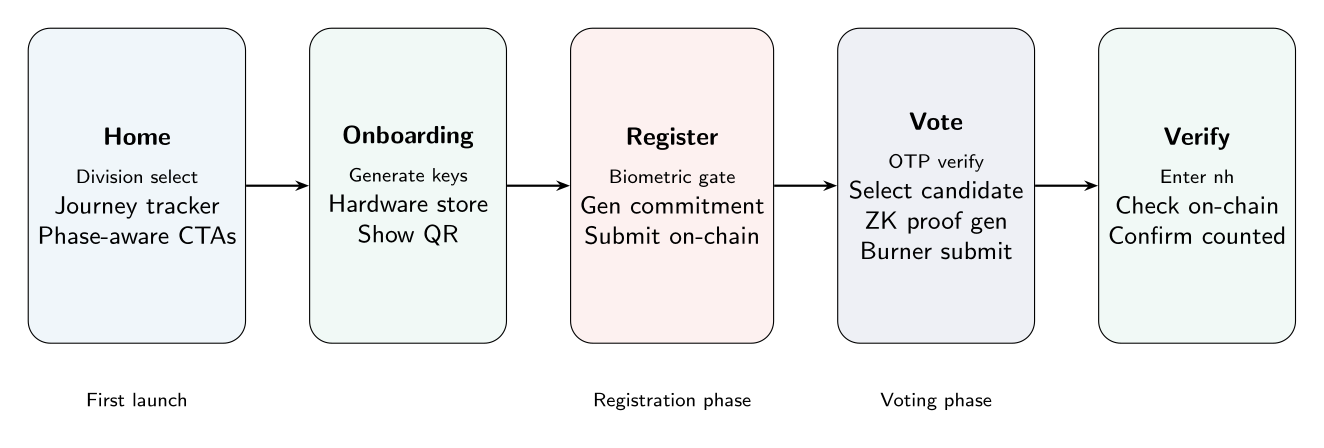
\includegraphics[width=0.85\textwidth]{Images/fig_mobile_flow.png}
\caption{Mobile app screen flow: from onboarding through registration to voting, with security gates at each transition.}
\label{fig:mobile-flow}
\end{figure}

\begin{table}[H]
\centering
\caption{Mobile app screen inventory.}
\label{tab:mobile-screens}
\begin{tabular}{|l|l|p{5cm}|}
\hline
\textbf{Route} & \textbf{Screen} & \textbf{Function} \\
\hline
\texttt{/} & Home & Division selector, journey tracker, action buttons \\
\hline
\texttt{/onboarding} & Onboarding & Identity creation (key generation) \\
\hline
\texttt{/register} & Registration & Biometric $\to$ Commitment $\to$ On-chain register \\
\hline
\texttt{/vote} & Voting & OTP $\to$ Biometric $\to$ Candidate $\to$ Proof $\to$ Submit \\
\hline
\texttt{/verify} & Verification & Check vote by nullifier hash \\
\hline
\texttt{/settings} & Settings & App configuration \\
\hline
\end{tabular}
\end{table}

\section{Hardware Keystore Implementation}

\subsection{Secure Storage Architecture}

\begin{figure}[H]
\centering
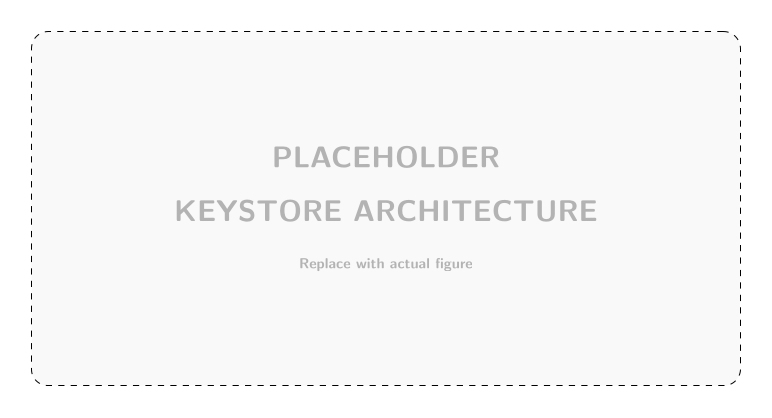
\includegraphics[width=0.85\textwidth]{Images/fig_keystore_architecture.png}
\caption{Hardware keystore architecture: sensitive secrets (private key, nullifier, secret) require biometric authentication; public data (address, flags) does not.}
\label{fig:keystore}
\end{figure}

The keystore separates items into two security tiers:

\begin{table}[H]
\centering
\caption{Keystore items with authentication requirements.}
\label{tab:keystore-items}
\begin{tabular}{|l|l|l|p{4cm}|}
\hline
\textbf{Key} & \textbf{Auth Gated} & \textbf{Type} & \textbf{Purpose} \\
\hline
\texttt{slvote.privateKey} & Yes (biometric) & Hex string & EVM transaction signing \\
\hline
\texttt{slvote.nullifier} & Yes (biometric) & Field element & ZK commitment secret \\
\hline
\texttt{slvote.secret} & Yes (biometric) & Field element & ZK commitment secret \\
\hline
\texttt{slvote.address} & No & Hex string & Public wallet address \\
\hline
\texttt{slvote.division} & No & Address & Selected division contract \\
\hline
\texttt{slvote.registered} & No & Boolean & Registration status flag \\
\hline
\texttt{slvote.voted} & No & JSON array & Divisions voted in \\
\hline
\end{tabular}
\end{table}

\subsection{Implementation Details}

\begin{lstlisting}[language=Java, caption={Keystore implementation with biometric gating.}]
import * as SecureStore from 'expo-secure-store';
import { Platform } from 'react-native';

const isExpoGo = Constants.appOwnership === 'expo';

const AUTH_OPTIONS: SecureStoreOptions = {
  requireAuthentication: !isExpoGo,
  authenticationPrompt: "Unlock your voting identity",
  keychainAccessible: 
    SecureStore.WHEN_UNLOCKED_THIS_DEVICE_ONLY,
};

// Biometric-gated access to private key
export async function getPrivateKey(): Promise<`0x${string}`> {
  const pk = await SecureStore.getItemAsync(
    'slvote.privateKey', AUTH_OPTIONS
  );
  if (!pk) throw new Error('No identity found');
  return pk as `0x${string}`;
}

// Public access (no biometric prompt)
export async function getAddress(): Promise<`0x${string}`> {
  const addr = await SecureStore.getItemAsync('slvote.address');
  return addr as `0x${string}`;
}
\end{lstlisting}

\subsection{Identity Creation}

\begin{lstlisting}[language=Java, caption={One-time identity creation during onboarding.}]
export async function createIdentity(): Promise<`0x${string}`> {
  // Generate cryptographic keypair
  const privateKey = generatePrivateKey(); // viem
  const address = privateKeyToAddress(privateKey);
  
  // Store with biometric protection
  await SecureStore.setItemAsync(
    'slvote.privateKey', privateKey, AUTH_OPTIONS
  );
  await SecureStore.setItemAsync('slvote.address', address);
  
  return address;
}
\end{lstlisting}

\section{Biometric Authentication Flow}

\begin{figure}[H]
\centering
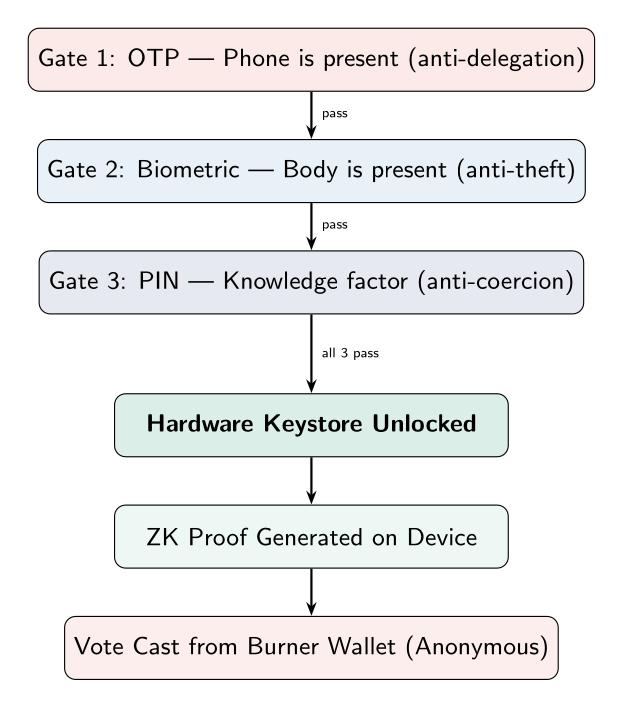
\includegraphics[width=0.85\textwidth]{Images/fig_auth.png}
\caption{Biometric authentication flow: capability check, enrollment verification, and hardware-backed prompt.}
\label{fig:auth-flow}
\end{figure}

\begin{lstlisting}[language=Java, caption={Biometric authentication with capability detection.}]
import * as LocalAuthentication from 'expo-local-authentication';

export async function authenticate(
  reason: string = "Verify your identity"
): Promise<boolean> {
  // Check hardware capability
  const hasHardware = await LocalAuthentication
    .hasHardwareAsync();
  if (!hasHardware) return false;
  
  // Check enrollment
  const isEnrolled = await LocalAuthentication
    .isEnrolledAsync();
  if (!isEnrolled) return false;
  
  // Prompt user
  const result = await LocalAuthentication
    .authenticateAsync({
      promptMessage: reason,
      fallbackLabel: "Use PIN",
      disableDeviceFallback: false,
    });
  
  return result.success;
}

export async function getBiometricCapability() {
  return {
    hasHardware: await LocalAuthentication.hasHardwareAsync(),
    isEnrolled: await LocalAuthentication.isEnrolledAsync(),
    supported: await LocalAuthentication
      .supportedAuthenticationTypesAsync(),
  };
}
\end{lstlisting}

\section{Commitment Cryptography}

\begin{lstlisting}[language=Java, caption={Voter commitment generation using Poseidon.}]
import { poseidon1, poseidon2 } from 'poseidon-lite';

const FIELD_PRIME = 21888242871839275222246405745257275088
  548364400416034343698204186575808495617n;

function randomFieldElement(): bigint {
  const bytes = crypto.getRandomValues(new Uint8Array(32));
  const num = BigInt('0x' + Buffer.from(bytes).toString('hex'));
  return num % FIELD_PRIME;
}

export interface VoterCommitment {
  nullifier: string;
  secret: string;
  commitment: string;
  nullifierHash: string;
}

export function generateCommitment(): VoterCommitment {
  const nullifier = randomFieldElement();
  const secret = randomFieldElement();
  const commitment = poseidon2([nullifier, secret]);
  const nullifierHash = poseidon1([nullifier]);
  
  return {
    nullifier: nullifier.toString(),
    secret: secret.toString(),
    commitment: commitment.toString(),
    nullifierHash: nullifierHash.toString(),
  };
}
\end{lstlisting}

\section{ZK Proof Generation on Mobile}

\subsection{WebView-Based Proving}

Due to Hermes's lack of BigInt support, ZK proof generation runs inside a React Native WebView that uses the device's system WebKit/Chromium engine (which supports BigInt natively):

\begin{lstlisting}[language=Java, caption={WebView proof generation architecture.}]
// React Native side: pass witness to WebView
const generateProof = async (inputs: CircuitInputs) => {
  return new Promise((resolve) => {
    webviewRef.current.postMessage(JSON.stringify({
      type: 'GENERATE_PROOF',
      inputs: inputs,
    }));
    
    // WebView will respond via onMessage
    onMessageRef.current = (event) => {
      const data = JSON.parse(event.nativeEvent.data);
      if (data.type === 'PROOF_RESULT') {
        resolve(data.proof);
      }
    };
  });
};

// WebView HTML (runs in system V8/JSCore):
// - Loads bb.js WASM module
// - Loads compiled ACIR circuit
// - Receives witness via postMessage
// - Generates UltraHonk proof
// - Returns proof bytes via postMessage
\end{lstlisting}

\subsection{Witness Construction}

\begin{lstlisting}[language=Java, caption={Circuit witness construction from voter secrets and chain state.}]
interface VoteProofParams {
  nullifier: string;
  secret: string;
  circuitIndex: string;   // Leaf index in tree
  siblings: string[];     // 16-element Merkle path
  root: string;           // Current tree root
  candidateIndex: number; // User's candidate choice
  depth: number;          // Current tree depth
}

function buildCircuitInputs(params: VoteProofParams): CircuitInputs {
  const nullifier = BigInt(params.nullifier);
  const nullifierHash = poseidon1([nullifier]);
  
  // Pad siblings to 16 elements
  const paddedSiblings = [...params.siblings];
  while (paddedSiblings.length < 16) {
    paddedSiblings.push("0");
  }
  
  return {
    nullifier_hash: nullifierHash.toString(),
    root: params.root,
    vote: params.candidateIndex.toString(),
    depth: params.depth.toString(),
    nullifier: params.nullifier,
    secret: params.secret,
    index: params.circuitIndex,
    siblings: paddedSiblings,
  };
}
\end{lstlisting}

\section{Chain Interaction: Legacy Transaction Signing}

\begin{lstlisting}[language=Java, caption={Manual legacy transaction signing for Hermes compatibility.}]
import { 
  encodeFunctionData, createWalletClient, http 
} from 'viem';

export async function submitVote(
  divisionContract: `0x${string}`,
  callData: VoteCallData,
  burnerPrivateKey: `0x${string}`,
): Promise<`0x${string}`> {
  // Encode vote function call
  const data = encodeFunctionData({
    abi: VotingABI,
    functionName: 'vote',
    args: [
      callData.proof,
      callData.nullifierHash,
      callData.root,
      callData.vote,
      callData.depth,
    ],
  });
  
  // Manual legacy tx (avoids BigInt gas estimation)
  const client = createWalletClient({
    account: privateKeyToAccount(burnerPrivateKey),
    transport: http(RPC_URL),
  });
  
  return client.sendTransaction({
    to: divisionContract,
    data: data,
    gas: 500000n,     // Fixed gas limit
    gasPrice: 0n,     // Gasless chain
    type: 'legacy',   // Avoid EIP-1559 BigInt issues
  });
}
\end{lstlisting}

\section{Three-Factor Voting Authentication}

The voting flow requires three independent authentication factors:

\begin{enumerate}
    \item \textbf{Factor 1: OTP Phone Verification}
    \begin{itemize}
        \item Voter enters phone number
        \item Server sends SMS OTP (6-digit code)
        \item Voter enters code within time window
        \item Prevents bot-based automated voting
    \end{itemize}
    
    \item \textbf{Factor 2: Biometric Authentication}
    \begin{itemize}
        \item Device fingerprint sensor or face recognition
        \item Hardware-backed (TEE/Secure Enclave)
        \item Unlocks access to voter secrets in keystore
        \item Proves physical possession of enrolled device
    \end{itemize}
    
    \item \textbf{Factor 3: Cryptographic Identity (Hardware PIN)}
    \begin{itemize}
        \item Private key stored in hardware keystore
        \item Only accessible after biometric + device PIN
        \item Used to sign the registration transaction
        \item Proves ownership of the registered commitment
    \end{itemize}
\end{enumerate}

\section{Burner Wallet Mechanism}

To achieve voter--ballot unlinkability, votes are submitted from ephemeral ``burner'' wallets:

\begin{lstlisting}[language=Java, caption={Burner wallet creation and usage.}]
export function newBurnerAccount() {
  const privateKey = generatePrivateKey();
  const address = privateKeyToAddress(privateKey);
  return { privateKey, address };
}

// Voting flow:
// 1. Generate fresh burner (no prior history)
// 2. Fund burner via faucet/paymaster (small amount for gas)
// 3. Submit vote from burner address
// 4. Discard burner private key (never stored)
\end{lstlisting}

\textbf{Key property}: The burner address has no transaction history linking it to the voter's registered address. Even if an observer correlates the faucet funding, the ZK proof prevents linking the proof to a specific voter identity.

\section{Next.js Web Application}

\subsection{Routes and Access Control}

\begin{table}[H]
\centering
\caption{Next.js web application routes.}
\label{tab:web-routes}
\begin{tabular}{|l|l|l|}
\hline
\textbf{Route} & \textbf{Purpose} & \textbf{Access} \\
\hline
\texttt{/} & Landing page & Public \\
\hline
\texttt{/voting} & Mobile download prompt & Public \\
\hline
\texttt{/voting/admin} & Election Authority dashboard & Admin wallet \\
\hline
\texttt{/voting/admin/[id]} & Division management & Admin wallet \\
\hline
\texttt{/gn} & Grama Niladhari portal & GN wallet \\
\hline
\texttt{/gn/register} & Voter enrollment & GN wallet \\
\hline
\texttt{/results} & Live election results & Public \\
\hline
\texttt{/audit} & Observer verification & Public \\
\hline
\texttt{/debug} & Contract debugging (dev only) & Dev \\
\hline
\end{tabular}
\end{table}

\subsection{Admin Dashboard}

\begin{figure}[H]
\centering
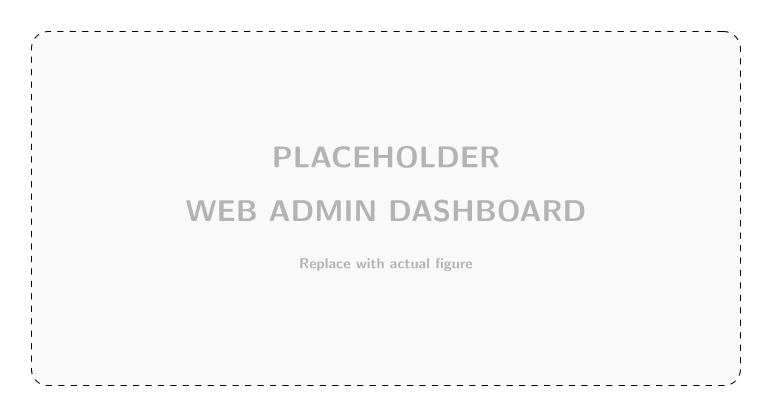
\includegraphics[width=0.85\textwidth]{Images/fig_web_admin_dashboard.png}
\caption{Web admin dashboard: division management, phase control, and national overview.}
\label{fig:admin-dashboard}
\end{figure}

The admin dashboard provides:
\begin{itemize}
    \item \textbf{Division Management}: Create divisions, assign GN officers, view per-division status
    \item \textbf{Election Setup}: Set ballot question, configure candidates (up to 100)
    \item \textbf{Phase Control}: Start registration/voting with configurable durations
    \item \textbf{National Overview}: Aggregate statistics across all 160 divisions
\end{itemize}

\subsection{GN Officer Portal}

\begin{figure}[H]
\centering
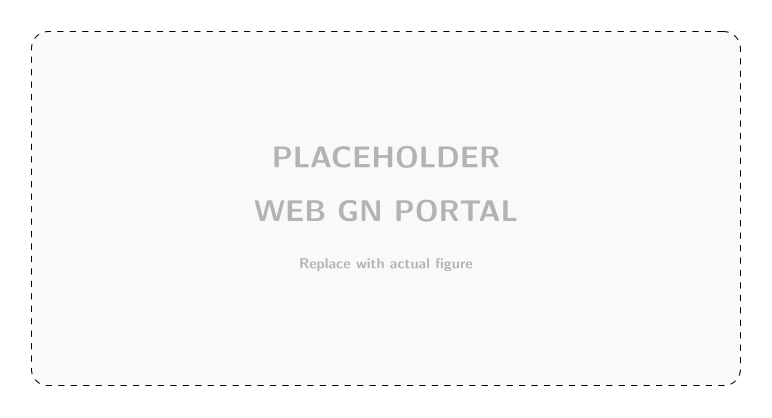
\includegraphics[width=0.85\textwidth]{Images/fig_web_gn_portal.png}
\caption{GN Officer portal: voter enrollment interface with QR scanning and NIC verification.}
\label{fig:gn-portal}
\end{figure}

The GN portal enables village officers to:
\begin{itemize}
    \item View their assigned division and its current phase
    \item Add voters to the allowlist (batch or individual)
    \item Monitor registration progress (tree size, voter list)
    \item Reserve NIC hashes for cross-division de-duplication
    \item Scan voter QR codes for identity verification
\end{itemize}

\subsection{Results Page and National Aggregation}

\begin{figure}[H]
\centering

\includegraphics[width=0.85\textwidth]{Images/fig_web_results_page.png}
\caption{Public results page: national vote totals with per-division breakdown and live updating.}
\label{fig:results-page}
\end{figure}

The results page provides:
\begin{itemize}
    \item National vote totals (pie chart + bar chart)
    \item Per-division breakdown (searchable table)
    \item Real-time polling (auto-refresh every 10 seconds)
    \item CSV export for independent analysis
    \item Turnout statistics (registered vs. voted)
\end{itemize}

\subsection{Dual Backend Architecture}

The web application supports two backends transparently:

\begin{lstlisting}[language=Java, caption={Backend-agnostic service layer configuration.}]
// scaffold.config.ts
const scaffoldConfig = {
  chainBackend: process.env.NEXT_PUBLIC_CHAIN_BACKEND 
    as "hardhat" | "custom",
  targetNetworks: [chains.hardhat],
  chainApiUrl: process.env.NEXT_PUBLIC_CHAIN_API_URL 
    || "http://localhost:3001",
};
\end{lstlisting}

\begin{table}[H]
\centering
\caption{Dual backend comparison: Hardhat vs. Custom Go blockchain.}
\label{tab:dual-backend}
\begin{tabular}{|l|l|l|}
\hline
\textbf{Aspect} & \textbf{Hardhat Backend} & \textbf{Custom Backend} \\
\hline
RPC & \texttt{localhost:8545} & \texttt{localhost:3001} (REST) \\
\hline
Voter ID & Ethereum address & String ID (email/phone) \\
\hline
Vote submission & Signed EVM tx & Unsigned POST /vote \\
\hline
Gas model & Standard gas & Gasless (free) \\
\hline
Admin auth & Contract ownership & RSA signature \\
\hline
\end{tabular}
\end{table}

This architecture allows development and testing on Hardhat (familiar tooling, fast iteration) while deploying to the custom blockchain for production (gasless, sovereign).

\section{Summary}

This chapter has detailed the complete application layer: a React Native mobile app with hardware-backed security, biometric authentication, and on-device ZK proof generation; and a Next.js web application with role-based access control for administrators, GN officers, and public observers. The three-factor authentication protocol (OTP + biometric + cryptographic identity) provides defense in depth for the voting action, while the burner wallet mechanism ensures voter--ballot unlinkability at the network layer. Chapter~\ref{ch:testing} evaluates the complete system's performance, security, and correctness through comprehensive testing.
